\documentclass[11pt,xcolor={dvipsnames},hyperref={pdftex,pdfpagemode=UseNone,hidelinks,pdfdisplaydoctitle=true},usepdftitle=false]{beamer}
\usepackage{presentation}
% Enter title of presentation PDF:
\hypersetup{pdftitle={Minimalist LaTeX Template for Academic Presentations}}
% Enter link to PDF file with figures:
\newcommand{\pdf}{figures.pdf}

\begin{document}
% Enter presentation title:
\title{Target-aware Variational Auto-encoders for Ligand Generation with Multimodal Protein Representation Learning}
\information%
[https://iopscience.iop.org/article/10.1088/2632-2153/ad3ee4]%
{Nhat Khang Ngo, Truong Son Hy}%
\frame{\titlepage}

\begin{frame}
    \frametitle{Introduction to Drug Discovery}
    Drug discovery is a critical, complex, and costly process that involves identifying molecular candidates that can effectively interact with specific biological targets. The process often spans several years and entails multi-stage experimentation and validation, with costs reaching into billions of dollars. The initial phase involves the discovery of novel drug-like compounds with high binding affinities to specific protein targets, leveraging techniques like virtual screenings and molecular dynamics simulations.
    % \cite{hughes2011principles, verkhivker2001binding, burley2019rcsb}
\end{frame}
    
% \begin{frame}
%     \frametitle{Challenges in Drug Discovery}
%     The primary challenges in the early stages of drug discovery include the vast chemical space of potential molecules, estimated at around $10^{33}$ chemically valid structures, and the computational expense of drug-target affinity (DTA) predictions. Traditional methods involve computationally intensive simulations that are impractical on a large scale, highlighting a crucial need for efficient computational techniques to predict and validate drug-likeness and binding affinities quickly.
%     % \cite{verkhivker2001binding, burley2019rcsb}
% \end{frame}
    
\begin{frame}
    \frametitle{Deep Generative Models for Drug Design}
    Deep generative models have been proposed to reduce the workload for wet-lab experiments by automating the generation and optimization of molecular properties. However, these models are often slow when enhancing binding affinity or other computationally expensive properties due to the need for reinforcement learning frameworks.
    
    % \cite{NEURIPS2018_d60678e8, pmlr-v80-jin18a, pmlr-v119-jin20a, luo2021a, Simonovsky2018GraphVAETG, de2018molgan, pmlr-v139-luo21a, gapsys2022pre, burley2019rcsb, verkhivker2001binding}
\end{frame}

\begin{frame}
    \frametitle{Protein Representation Learning}
    Proteins can be represented as sequences of amino acids, 2D graphs at residue level, or 3D point clouds at atom level. Advanced methods leverage language models (sequential modal), graph neural networks (GNNs), and convolutional neural networks (CNNs) (graph modal) to learn from these representations.
    
    % \cite{pmlr-v162-notin22a, 10.1093/bioinformatics/btac020, asgari2019probabilistic, WU202118, 10.1093/bioinformatics/bty178, NEURIPS2019_03573b32, townshend2020atom3d, jing2021equivariant, jing2021learning, 10.1093/nargab/lqac004}
\end{frame}

\begin{frame}
    \frametitle{Contributions}
    \begin{itemize}
        \item Developed \textbf{TargetVAE}, a conditional VAE model to generate drug-like molecules with high binding affinity to given protein structures.
        \item Adapted techniques from computer vision to transfer weights from an unconditional to a conditional VAE, enhancing molecule generation diversity.
        \item Introduced \textbf{Protein Multimodal Network (PMXN)}, which unifies sequence and structural modalities of proteins for improved prediction of binding affinities.
    \end{itemize}
\end{frame}

\begin{frame}
    \frametitle{Background: Rotational Invariant Features}
    Geometric features of protein structures can be represented as tuples of scalar and vector features, which are respectively invariant and equivariant to geometric transformations in Euclidean space. The Geometric Vector Perceptron (GVP) is used to transform input features, ensuring the desired properties of invariance and equivariance.
    
    % \cite{jing2021learning}
\end{frame}

\begin{frame}
    \frametitle{Variational Auto-Encoders (VAEs)}
    VAEs consist of a generative model and an inference model, using a probabilistic decoder and a prior to define a joint distribution between latent variables and data. Conditional VAEs integrate auxiliary covariates to enhance generative modeling, trained to maximize the conditional evidence lower bound (ELBO).
    
    % \cite{kingma2013auto, NIPS2015_8d55a249, Zheng_2019_CVPR, ivanov2018variational, wan2021high}
    \begin{figure}[t]
        \centering
        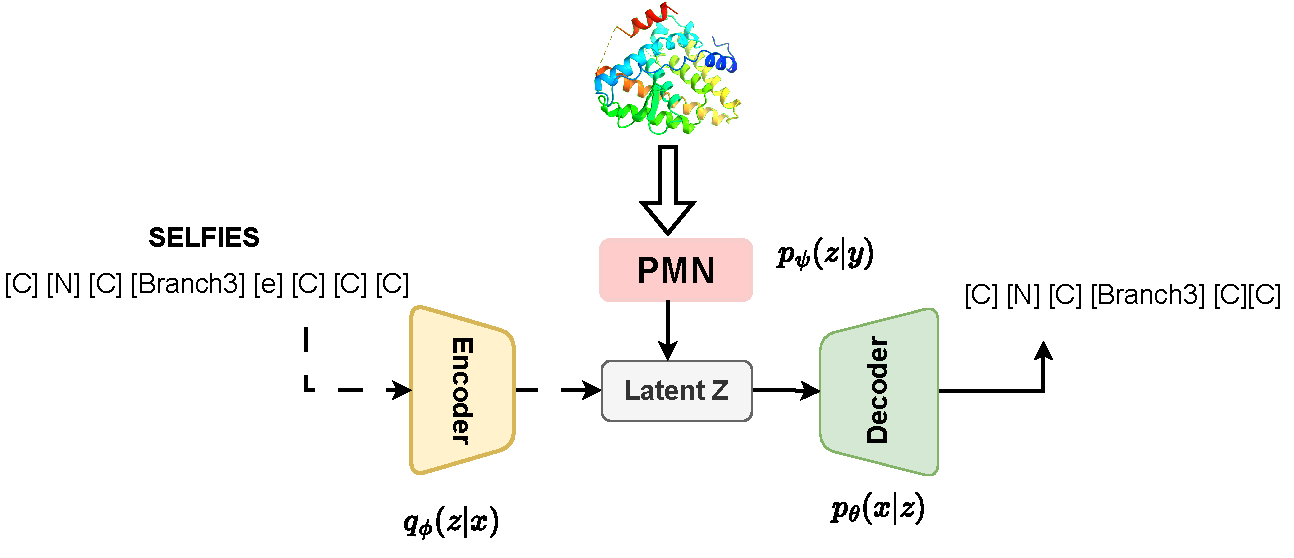
\includegraphics[width = 10cm]{./media/_vae_4_protein/target_vae.pdf}
        \caption{VAE}
    \end{figure}
\end{frame}
    

\begin{frame}
    \frametitle{Protein Multimodal Network (PMN): Overview}
    \textbf{Objective:} Integrate diverse protein representations into a unified framework capable of capturing both local and global structural features, utilizing advanced graph and sequence modeling techniques.
    
    % On the graph, nodes and edges are attributed by scalar and vector features $(s, V)$, which are propagated on the graph via a message-passing network with GVP modules. The processed invariant features $s$ are then moved to an efficient Transformer encoder to learn pairwise relations between residues. For sequence modeling, each residue is regarded as a token in the long protein sequence, and an efficient Transformer-based language model is used to learn their representations. Representations of residues are aggregated to produce representation vectors for the entire protein in both pipelines; then, these two vectors are concatenated and moved to dense layers to obtain the final representation.
    
    \begin{figure}[t]
        \centering
        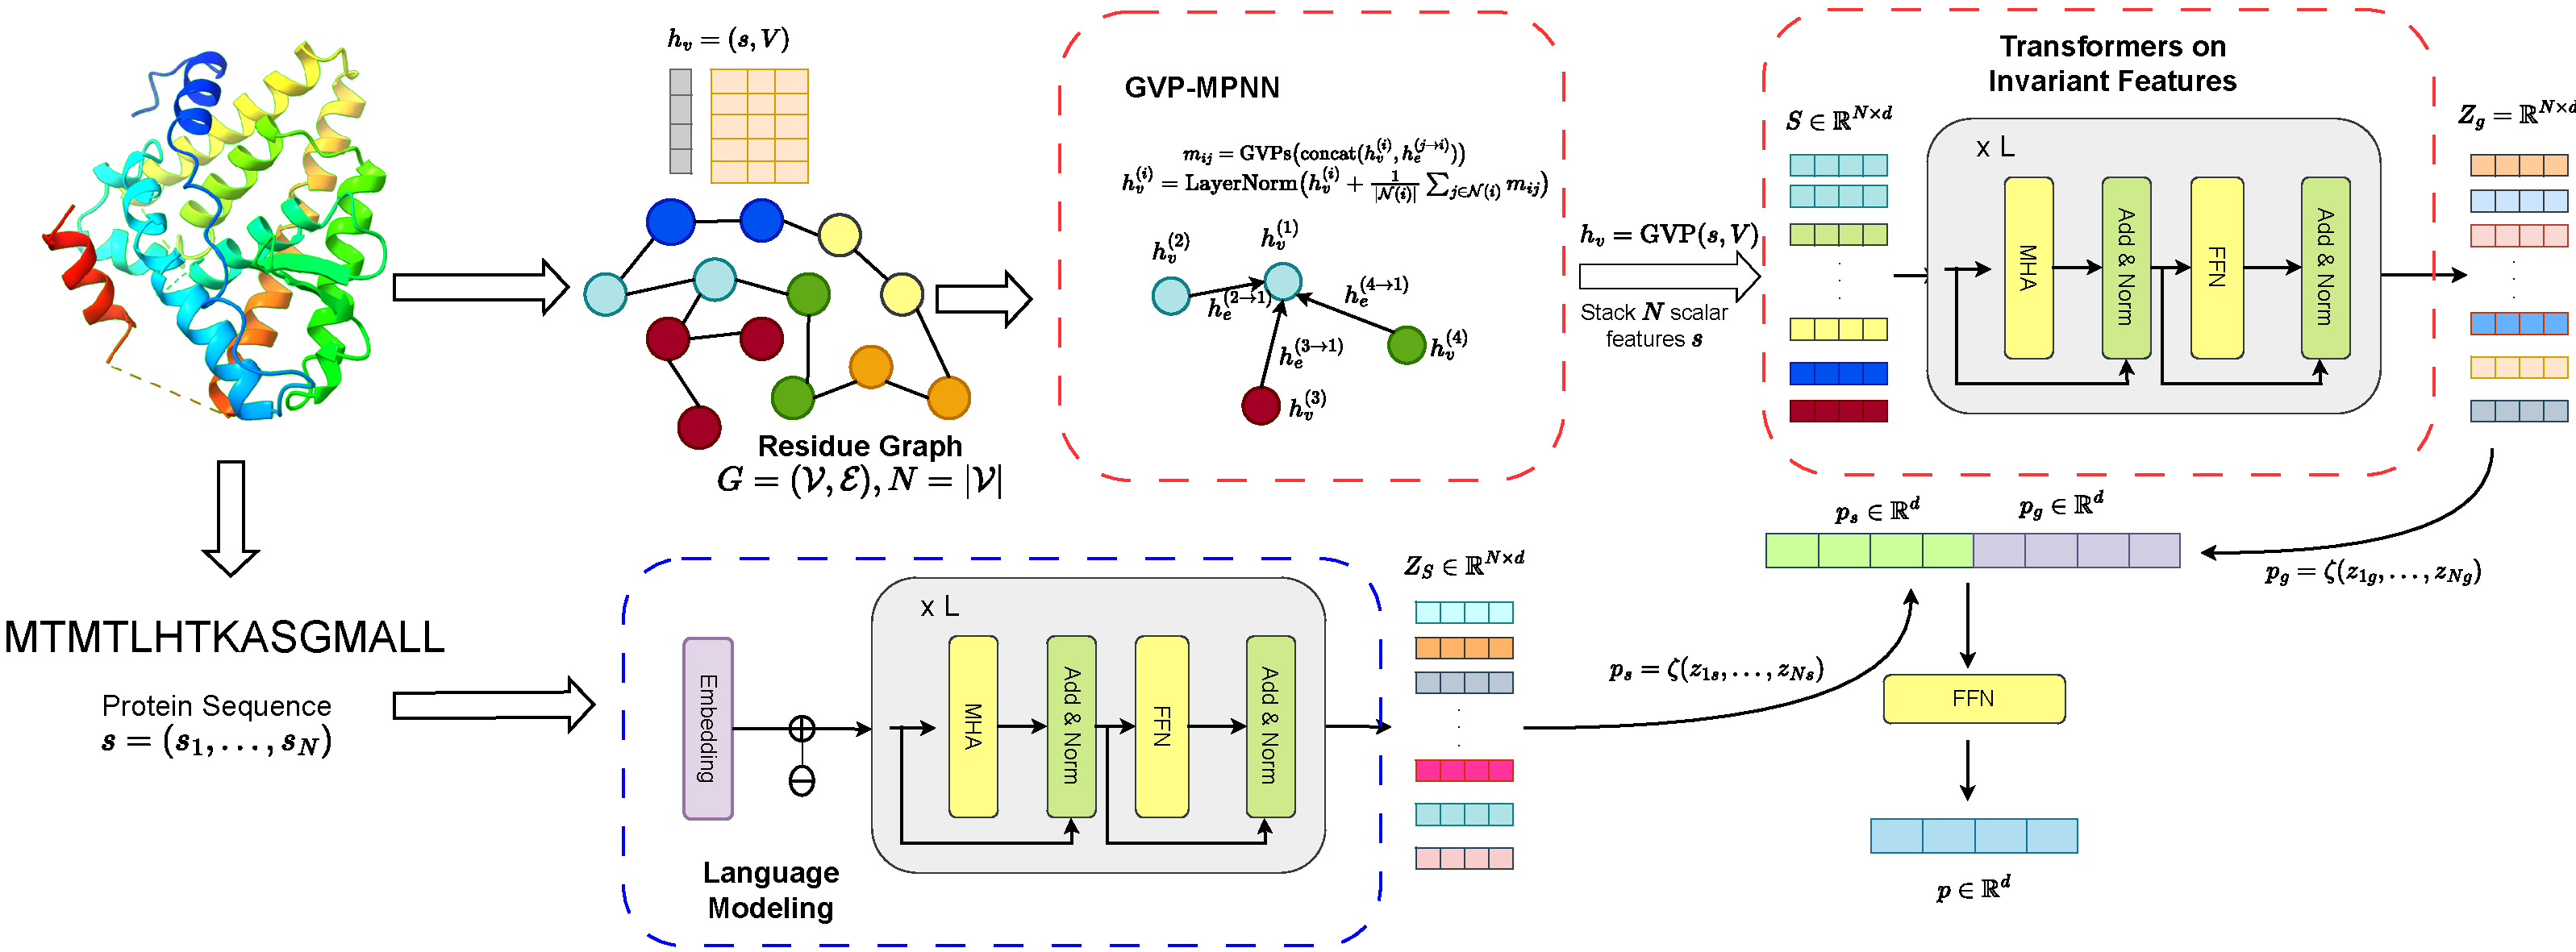
\includegraphics[width = 10cm]{./media/_vae_4_protein/pmn.pdf}
        \caption{Overview of Protein Multimodal Network (PMN).}
    \end{figure}
\end{frame}

\begin{frame}
\frametitle{Long-range Modeling on 3D Structures}
\textbf{Key Components:}
\begin{itemize}
    \item Local Encoder: Uses GVPs to update node features based on their scalar and vector attributes.
    \item GVP Module: Transforms features to maintain rotational invariance and equivariance.
    \item Global Transformer Encoder: Captures long-range interactions using self-attention mechanisms.
\end{itemize}

\textbf{Mathematical Formulation:}
\begin{align*}
    m_{ij} &= \text{GVPs}\left(\text{concat}(h_v^{(i)}, h_e^{(j \rightarrow i)})\right), \\
    h_v^{(i)} &= \text{LayerNorm}\left(h_v^{(i)} + \frac{1}{|\mathcal{N}(i)|}\sum_{j \in \mathcal{N}(i)} m_{ij}\right).
\end{align*}

% Where $m_{ij}$ computed by a module of three GVP layers denotes the message propagated from node $j$ to $i$. Also, $h_v^{(i)}$ and $h_e^{(j \rightarrow i)}$ indicate the embeddings of node $i$ and edge $(j \rightarrow i)$ and are tuples of scalar and vector features as described in Section \ref{background:rotation_invariant}.
\end{frame}

\begin{frame}
\frametitle{Language Modeling on Protein Sequence}
\textbf{Approach:}
\begin{itemize}
    \item Utilize Transformer-based models to process sequences where each residue is treated as a token.
    \item Embedding layers transform residue tokens into dense vector representations, incorporating positional encodings.
\end{itemize}

\textbf{Transformations:}
\begin{align*}
    Q_\ell &= Z_{\ell-1} W_\ell^Q, \quad K_\ell = Z_{\ell-1} W_\ell^K, \quad V_\ell = Z_{\ell-1} W_\ell^V, \\
    H_\ell &= \text{MultiheadAttention}(Q_\ell, K_\ell, V_\ell), \\
    Z_\ell &= \text{LayerNorm}(Z_{\ell-1} + \text{FFN}(H_\ell)).
\end{align*}

% Here, $Z_0$ is initialized to the sequence embeddings; $W_\ell^Q, W_\ell^K, W_\ell^V$ are learnable weight matrices for the query, key, and value in the Transformer's self-attention mechanism.
\end{frame}

\begin{frame}
\frametitle{Unified Representation and Protein Embedding}
\textbf{Final Integration:}
\begin{itemize}
    \item Aggregated embeddings from both the graph and sequence models are concatenated.
    \item The concatenated vector is passed through dense layers to produce the final representation of the protein.
\end{itemize}

\textbf{Representation Output:}
\begin{equation*}
    p = W_2 \text{ReLU}(W_1 (\text{concat}(p_g, p_s)) + b_1) + b_2
\end{equation*}

% Where $p_g$ and $p_s$ are the aggregated graph and sequence representations, respectively.
\end{frame}


% Remove experiment result (add 1,2 lines into the first slide). create an overview slides of all experiments

\begin{frame}
\frametitle{Binding Affinity Prediction}
\textbf{Datasets:}
\begin{itemize}
    \item \textbf{DAVIS} - 442 proteins and 68 ligands, 30,056 pairs. $K_D$ constants.
    \item \textbf{KIBA} - 229 proteins and 2,111 ligands, 118,254 pairs. KIBA scores.
\end{itemize}
\textbf{Data Enhancement:} 3D protein structures generated by AlphaFold included for a comprehensive dataset. \\
\textbf{Evaluation Metrics:} Mean Squared Error (MSE), Concordance Index (CI), and $r_m ^ 2$ Index. \\
\textbf{Result:} Superior performance on DAVIS and competitive on KIBA against benchmarks KronRLS, SimBoost, and GraphDTA.

% \textbf{Results Visualization:}
% \begin{figure}
%     \centering
%     \includegraphics[width=0.8\linewidth]{images/results_davis_kiba.png} % Example path to image
%     \caption{Performance on DAVIS and KIBA datasets across different models.}
% \end{figure}
\end{frame}

\begin{frame}
\frametitle{Target-aware Drug Design}
\textbf{Dataset for Drug Design:} Utilize KIBA and ZINC250K datasets for training conditional molecule generation models. \\
\textbf{Techniques:}
\begin{itemize}
    \item Models trained to generate SELFIES representations of molecules.
    \item Evaluate using Fréchet ChemNet Distance (FCD) and other chemical properties (QED, pLogP, SA).
\end{itemize}
\textbf{Advanced Evaluation:} Docking measurements using AutoDock-GPU for binding affinity predictions.

\textbf{Generative Model Quality:}
\begin{itemize}
    \item Low FCD scores indicating close approximation to real molecular distributions.
    \item Generated molecules showcase desirable drug-like properties.
\end{itemize}
% \textbf{Visualization of Generated Molecules:}
% \begin{figure}
%     \centering
%     \includegraphics[width=0.8\linewidth]{images/generated_molecules.png} % Example path to image
%     \caption{Molecules generated for targets ESR1 and ACAA1.}
% \end{figure}
\end{frame}

\begin{frame}
\frametitle{Binding Experiments with Unseen Targets}
\textbf{Experiment Details:}
\begin{itemize}
    \item Testing on unseen targets shows our model's ability to generalize and effectively predict binding affinities.
    \item Comparison with state-of-the-art models demonstrates superior or comparable performance.
\end{itemize}
\textbf{Results Discussion:}
\begin{itemize}
    \item Highlights advantages of our method in balancing binding affinities and drug-like properties.
    \item Provides insight into the potential for zero-shot learning capabilities in drug discovery.
\end{itemize}
\end{frame}

\end{document}